\documentclass[../main.tex]{subfiles}


\begin{document}

\section{Introduzione}
L'approssimazione è il processo di costruzione di una curva che coincida il più possibile con dei  dati soggetti ad errore casuale.
Queste tecniche vengo usate come alternativa all'interpolazione, dove si vuole un'esatta corrispondenza con alcuni punti dati.
Ci sono delle situazioni in cui è conveniente usare tecniche di approssimazione, ad esempio:
\begin{enumerate}
    \item visualizzazione dei dati
    \item rappresentazione di una funzione dove non sono disponibili dati
    \item sintetizzare relazioni tra variabili
\end{enumerate}
Ci sono vari campi che utilizzano tecniche di approssimazione ad esempio la \textit{modellazione statistica}, \textit{machine learning} e 
\textit{statistical learning}, ma con obbiettivi diversi.
Il nostro obbiettivo è quello di fornire un'approssimazione il più possibile precisa di dati generati da funzioni generatrici, soggetti ad errori casuali.
Non ci interessa quindi l'interpretazione dei risultati ottenuti.
Nel seguito useremo i dati generati casualmente mostrati in tabella \ref{tab:Dati}.

\begin{table}
    \centering
    \caption{Dati generati.\label{tab:Dati}}
        \begin{tabular}{ccc}
             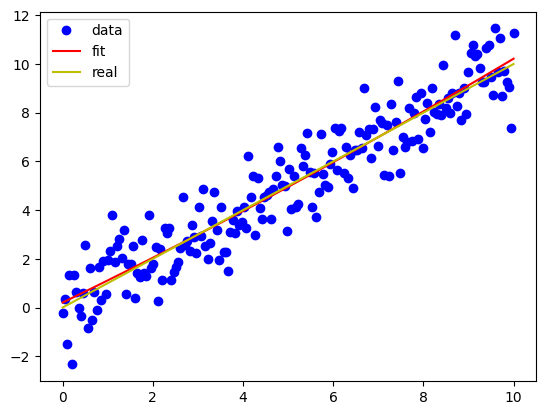
\includegraphics[width=0.45\linewidth]{Immagini/Introduzione/retta.png}
            & 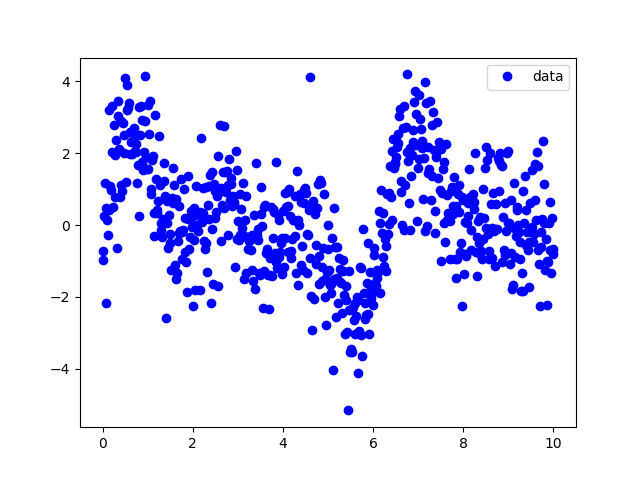
\includegraphics[width=0.45\linewidth]{Immagini/Introduzione/seno_complesso.png}\\[-4pt]
            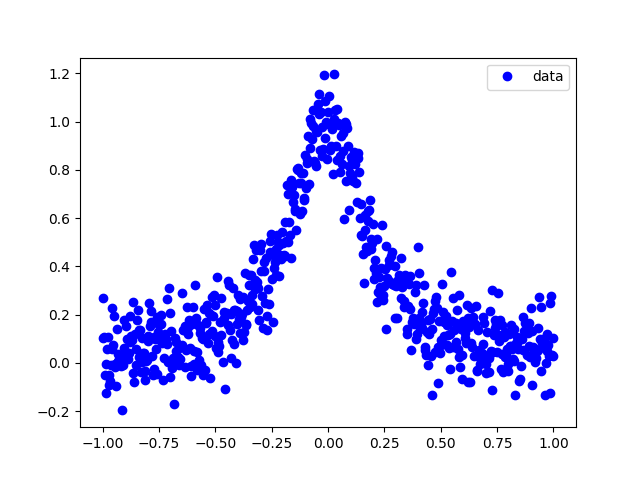
\includegraphics[width=0.45\linewidth]{Immagini/Introduzione/runge.png}
            &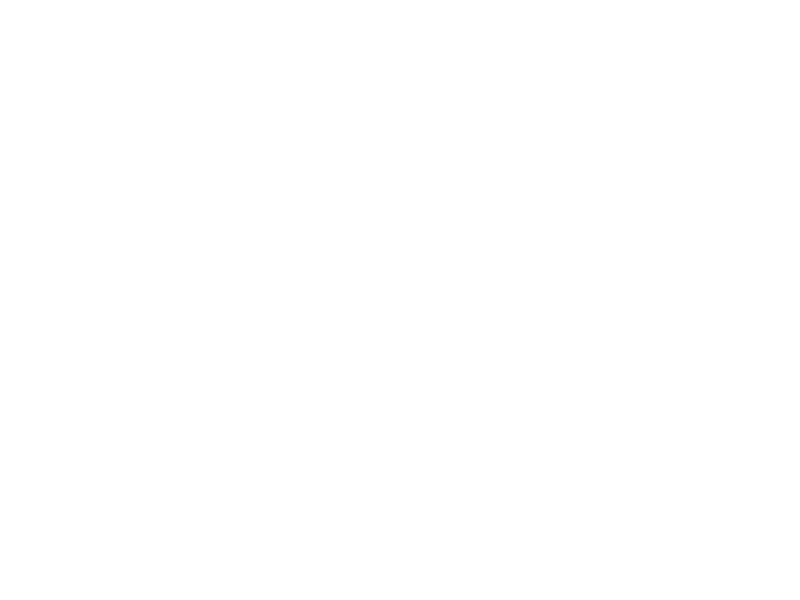
\includegraphics[width=0.45\linewidth]{Immagini/blank.png}\\[-4pt]
        \end{tabular}%
        \caption{Funzioni generatrici utilizzate: $y = x + \varepsilon$,  $\sin{2x} + \sin{3x} + \varepsilon$,  $\frac{1}{1+25x^2} + \varepsilon$ ($\varepsilon\sim N(0,0.1) $)}
\end{table}


\end{document}